\documentclass{article}
\usepackage[
        a4paper,
        left=3cm,
        right=3cm,
        top=3cm,
        bottom=4cm,
]{geometry}
\usepackage{graphicx}
\usepackage{caption}
\usepackage{enumerate}
\usepackage{subcaption}
\usepackage[procnames]{listings}
\usepackage{color}
\usepackage{amsmath}
\usepackage{hyperref}
\usepackage[at]{easylist}
\title{Lab Assignement 1}
\date{\today}
\author{
	Karamoulas Eleftherios - S3261859\\
	Tzafos Panagiotis - S3302148\\
}

\begin{document}
\maketitle
\section{Answers for Lab 1 sections 5,6}
\begin{enumerate}[{5.a}]
  \item The error is not decreasing in each epoch because in some iterations with the weight changes the output is the desired one.
  \item Because in the case of goal/output 1/0 and 0/1 even though the error should be the same we have 1 and -1 thats why we use the square.
  \item Because the required iterations to reach 0 depend on the random starting values and the learn rate that we use.
  \item With learning rate 0.6 we observe that more epochs are required to reach 0 error. Using higher learning rate is not always good. The learning rate that should be used depends on the training set.
  \item The TLU is still capable of learning the AND-function after both changes however when we have 0.2 and 0.8 in some cases it needs more epochs to reach 0 error.
  \item In sub-question 5.e we encountered with Resilience to noise our artificial neural network checks if the weighted summation of the inputs is above or below the threshold no matter the difference so small changes in the inputs or the weights don't lead to changes.
  \item TLU can learn the NAND-function however both weights and threshold become negative because the NAND is exactly the opposite of AND so the weights and the threshold are from the other side.
\begin{figure}[!h]
    \centering
    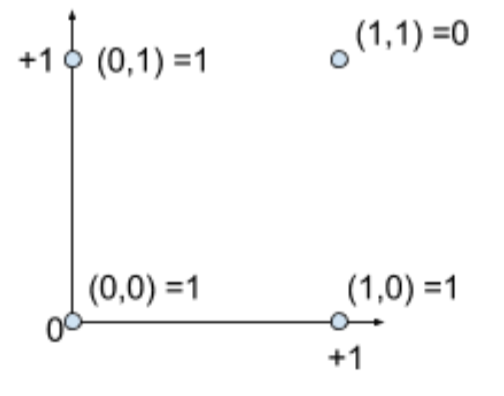
\includegraphics[width=0.5\textwidth]{img/nand.png}
    \caption{NAND}
    \label{fig:diagram}
  \end{figure}
\end{enumerate}
\begin{enumerate}[{6}]
  \item We observe that the weights, threshold and errors change all the time because the TLU can’t solve nonlinear separable problems and XOR is one of them because of the positions that 1 and 0 have in the coordinate system we can’t a line that separates the outputs in two planes.
  \begin{figure}[!h]
    \centering
    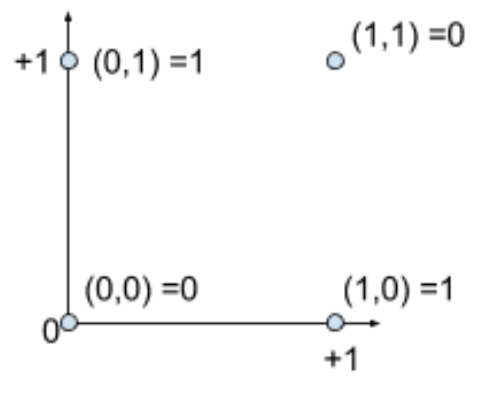
\includegraphics[width=0.5\textwidth]{img/xor.png}
    \caption{XOR}
    \label{fig:diagram}
  \end{figure}
\end{enumerate}
\section{Code for TLU}
\lstinputlisting[caption={tlu.m},label={code:bar}]{tlu.m}
\end{document}